\begin{problem}{게임말 올려놓기}{standard input}{standard output}{1 second}{1024 megabytes}

가로 $N$칸, 세로 $M$칸으로 이루어진 직사각형 모양의 게임판이 있다. 똑같은 게임말 두 개를 서로 대각선으로 이웃하게 올려두는 방법의 수를 출력하시오.

아래 그림은 $N = 3$, $M = 2$인 경우의 예시이다.
\begin{center}
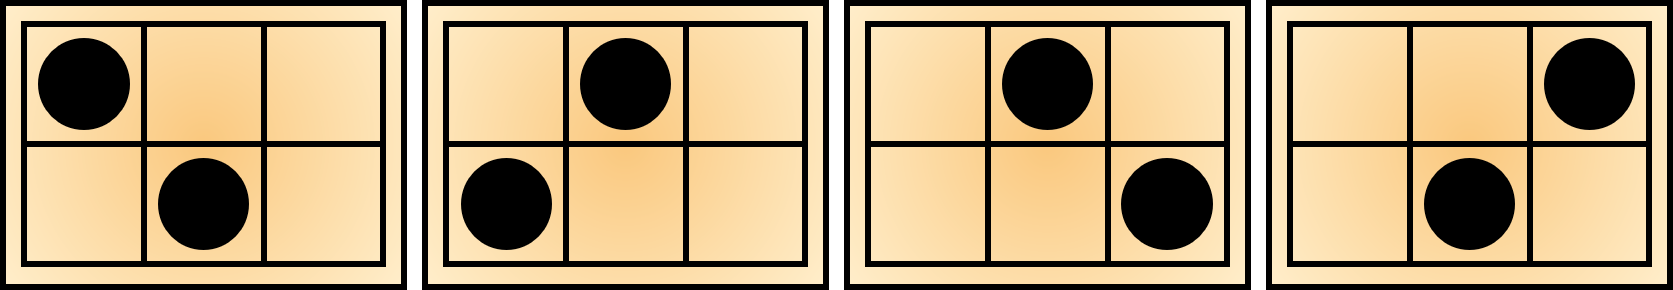
\includegraphics{grid.png}
\end{center}

\InputFile
첫 번째 줄에 바둑판의 가로 길이 $N$이 주어진다. $(1 \le N \le 40)$

두 번째 줄에 바둑판의 세로 길이 $M$이 주어진다. $(1 \le M \le 40)$

\OutputFile
위 조건을 만족하도록 게임말을 두는 경우의 수를 출력한다.

\Examples

\begin{example}
\exmpfile{example.01}{example.01.a}%
\exmpfile{example.02}{example.02.a}%
\exmpfile{example.03}{example.03.a}%
\end{example}

\Note
첫 번째 예시의 모든 경우의 수는 위의 그림과 같다.

두 번째 예시에서는 두 게임말을 대각선으로 이웃하게 올려둘 수 없으므로, 정답은 $0$이다.

\end{problem}

